\graphicspath{{chapters/gradient_descent/}}


\chapter{Efficient Algorithms for the CCA Family: Unconstrained Losses with Unbiased Gradients}\label{ch:gradient_descent}
\epigraph{It seems easier to train a bi-directional LSTM with attention than to compute the SVD of a large matrix}{Chris Ré}\citep{gemp2021}
\minitoc
% chktex-file 44
% chktex-file 3
\section*{Preface}
The content of this chapter is based on a series of papers~\citep{chapman2022generalized, chapman2023efficient} as well as a NeurIPS workshop paper~\citep{chapman2023cca}.
I am grateful to my co-authors Lennie Wells and Ana Lawry Aguila for their contributions to this work.
In particular, Lennie's mathematical expertise improved the theoretical grounding of the idea greatly and Ana's access to the UK Biobank dataset enabled the application of our methods to a real-world biomedical dataset.
In this thesis I include much of the work from these papers, but I exclude many of Lennie's extensive proofs where I can make no claim to have contributed beyond proofreading.

\section{Introduction}

Classical algorithms for linear CCA methods require computing full covariance matrices and so scale quadratically with dimension, becoming intractable for many large-scale datasets of practical interest.
There is therefore great interest in approximating solutions for CCA in stochastic or data-streaming settings \citep{arora2012stochastic}.

In this chapter, we propose a novel approach to solving the Generalized Eigenvalue Problem (GEP) for CCA and related methods.
Our method is based on a novel objective function inspired by the Eckhart--Young--Minsky inequality \citep{stewart_matrix_1990}.
We show that this objective has no spurious local minima and can be optimized efficiently using stochastic gradient descent.
We apply this method to CCA and Partial Least Squares (PLS), and show that it can outperform existing methods in terms of convergence speed and robustness to hyperparameter settings.

\section{Background: Solutions to CCA}\label{sec:background-unified}

\subsection{Solving High-Dimensional Generalized Eigenvalue Problems}

The GEP is often represented as \( Au = \lambda Bu \), where \( A \) and \( B \) are matrices. To generalize the dimensions of these matrices, let's denote them as \( m \times m \). This dimension \( m \) can vary based on the specific method in use. For instance, in Principal Component Analysis (PCA), represented as \acrshort{pca}, \( m \) would be equal to \( p \) since \( A \) and \( B \) are \( p \times p \) matrices. In methods like Partial Least Squares (PLS) and Canonical Correlation Analysis (CCA), represented as \acrshort{pls} and \acrshort{cca} respectively, \( m \) would be \( p_1+p_2 \), as \( A \) and \( B \) in these cases are \( (p_1+p_2) \times (p_1+p_2) \).


\subsection{Unified GEP formulation for CCA, Ridge CCA, PLS, and PCA} 
As discussed in \ref{ch:background}\ref{sec:classical-subspace-learning-algorithms}, we can formulate a unified framework for CCA, ridge-regularized CCA, and PLS using a generalized eigenvalue problem (GEP). This framework involves block matrices $A,B_\alpha \in \R^{D \times D}$, where the diagonal blocks of $A$ are zero, the off-diagonal blocks of $B_\alpha$ are zero, and the remaining blocks are defined as:

\begin{align}
A^{(ij)} &= \Cov(X\sps{i}, X\sps{j}) \text{ for } i \neq j, \\
B_\alpha^{(ii)} &= \alpha_i I_{D\sps{i}} + (1-\alpha_i) \Var(X\sps{i}),
\end{align}

where $\alpha \in [0,1]^I$ is a vector of ridge penalty parameters. By adjusting the values of $\alpha$, we can recover various subspace learning methods:

\begin{itemize}
\item Pure CCA: Setting $\alpha_i = 0 : \forall i$ recovers the classic CCA problem.
\item Ridge Extensions: Smoothly transition to ridge-regularized CCA or PLS by selectively adjusting values within \(\alpha\).
\item PCA Subsumption: Even PCA emerges as a special case – a single-view form of ridge-regularized PLS.
\end{itemize}

Crucially, this unification allows us to focus on solving the core CCA problem for the remainder of the chapter. The insights and solutions we develop will naturally generalize to the entire family of CCA, PLS, ridge-regularized extensions, and even PCA.

% Table \ref{tab:subspace} provides a comprehensive overview of the definitions and dimensions of \( A \) and \( B \) for various subspace learning methods. 

% \begin{table}[h]
%     \centering
%     \tiny
%     \begin{tabular}{|c|c|c|c|c|}
%         \hline
%         Method         & \( A \)           & \( B \)   & \( u \)        & Dimensions       \\
%         \hline
%         PCA & \( \Sigma_{11} \) & \( I \)   & \( u\sps{1} \) & \( p \times p \) \\
%         \hline
%         CCA & \( \begin{pmatrix} \Sigma_{11} & \Sigma_{12} \\ \Sigma_{21} & \Sigma_{22} \end{pmatrix} \) & \( \begin{pmatrix} \Sigma_{11} & 0 \\ 0 & \Sigma_{22} \end{pmatrix} \) & \( \begin{pmatrix} u\sps{1} \\ u\sps{2} \end{pmatrix} \) & \( (p_1+p_2) \times (p_1+p_2) \) \\
%         \hline
%         PLS & \( \begin{pmatrix} 0 & \Sigma_{12} \\ \Sigma_{21} & 0 \end{pmatrix} \) & \( I \) & \( \begin{pmatrix} u\sps{1} \\ u\sps{2} \end{pmatrix} \) & \( (p_1+p_2) \times (p_1+p_2) \) \\
%         \hline
%         Ridge CCA   & \( \begin{pmatrix} \Sigma_{11} & \Sigma_{12} \\ \Sigma_{21} & \Sigma_{22} \end{pmatrix} \) & \( \begin{pmatrix} \alpha_1 I + (1-\alpha_1)\Sigma_{11} & 0 \\ 0 & \alpha_2 I + (1-\alpha_2)\Sigma_{22} \end{pmatrix} \) & \( \begin{pmatrix} u\sps{1} \\ u\sps{2} \end{pmatrix} \) & \( (p_1+p_2) \times (p_1+p_2) \) \\
%         \hline
%         MCCA &   \( \begin{pmatrix} 0 & \Sigma_{12} & \cdots & \Sigma_{1m} \\ \Sigma_{21} & 0 & \cdots & \Sigma_{2m} \\ \vdots & \vdots & \ddots & \vdots  \\ \Sigma_{m1} & \Sigma_{m2} & \cdots & 0 \end{pmatrix} \) &  \(    \begin{pmatrix} \Sigma_{11} & 0 & \cdots & 0  \\ 0 & \Sigma_{22} & \cdots & 0  \\ \vdots & \vdots & \ddots & \vdots \\ 0 & 0 & \cdots & \Sigma_{mm} \end{pmatrix} \) & \( \begin{pmatrix}  u\sps{1} \\ u\sps{2} \\ \vdots \\ u\sps{m} \end{pmatrix} \) & \( \sum_{i=1}^I p_i \times \sum_{i=1}^I p_i \)    \\
%         \hline
%     \end{tabular}
%     \caption{Definitions and dimensions of \( A \) and \( B \) for different subspace learning methods.}
%     \label{tab:subspace}
% \end{table}

\subsection{Classical Methods for Solving CCA}

\subsubsection{Direct Solution}

To solve the GEP, one common technique is to transform it into a standard eigenvalue problem \( B^{-\frac{1}{2}} A B^{-\frac{1}{2}} y = \lambda y \), followed by eigendecomposition.
However, this approach has computational complexity \( \mathcal{O}((p_1+p_2)^3) \) and may suffer from numerical instability.

\subsubsection{\acrshort{pca}-CCA}

One way to reduce the complexity of solving GEPs is to use the \acrshort{pca}-CCA method, which first applies \acrshort{pca} to the data and then solves the GEP in the reduced space.
An important advantage of using \acrshort{pca}-CCA is computational efficiency, especially for high-dimensional data.
The overall complexity of \acrshort{pca}-CCA involves two main steps.
First, applying PCA has a complexity of \( \mathcal{O}(p_1^3+ p_2^3) \), dominated by the larger of the two matrices.
Second, solving the generalized eigenvalue problem in the reduced space with \( K \) components in each view leads to a complexity of \( \mathcal{O}((2K)^3) \).
Thus, the overall complexity of \acrshort{pca}-CCA is \( \mathcal{O}(p_1^3+ p_2^3) + (2K)^3) \), which is significantly lower than the complexity of solving the GEP directly.
Since CCA, ridge CCA, and PLS can all be solved in the principal component space, \acrshort{pca}-CCA can be used to compute solutions efficiently \textit{even if we keep all the principal components}.
Most obviously, this is the case when the number of samples \( n \) is smaller than either of the number of features \( p_1 \) or \( p_2 \), i.e. \( n < p_1 \) or \( n < p_2 \).
In this case the maximum number of principal components is \( K=n \), and the complexity of PCA is \( \mathcal{O}(n^3+ n^3) \) so that the overall complexity of \acrshort{pca}-CCA is thus \( \mathcal{O}(2n^3+(2n^3)^3) \) = \( \mathcal{O}(10n^3) \).
For fat data where \( p_1 \) and \( p_2 \) are larger than \( n \), we can reasonably expect $10n^3<p_1^3+ p_2^3$ and thus \acrshort{pca}-CCA is still more efficient than solving the original GEP.

We illustrate this in a simple simulation study in Figure \ref{fig:pca-cca-complexity}\footnote{This simulation was used to justify our pull request to \texttt{scikit-learn}\citep{pedregosa2011scikit} implementing a PCA-PLS and PCA-CCA backend}.

 \begin{figure}
     \centering
     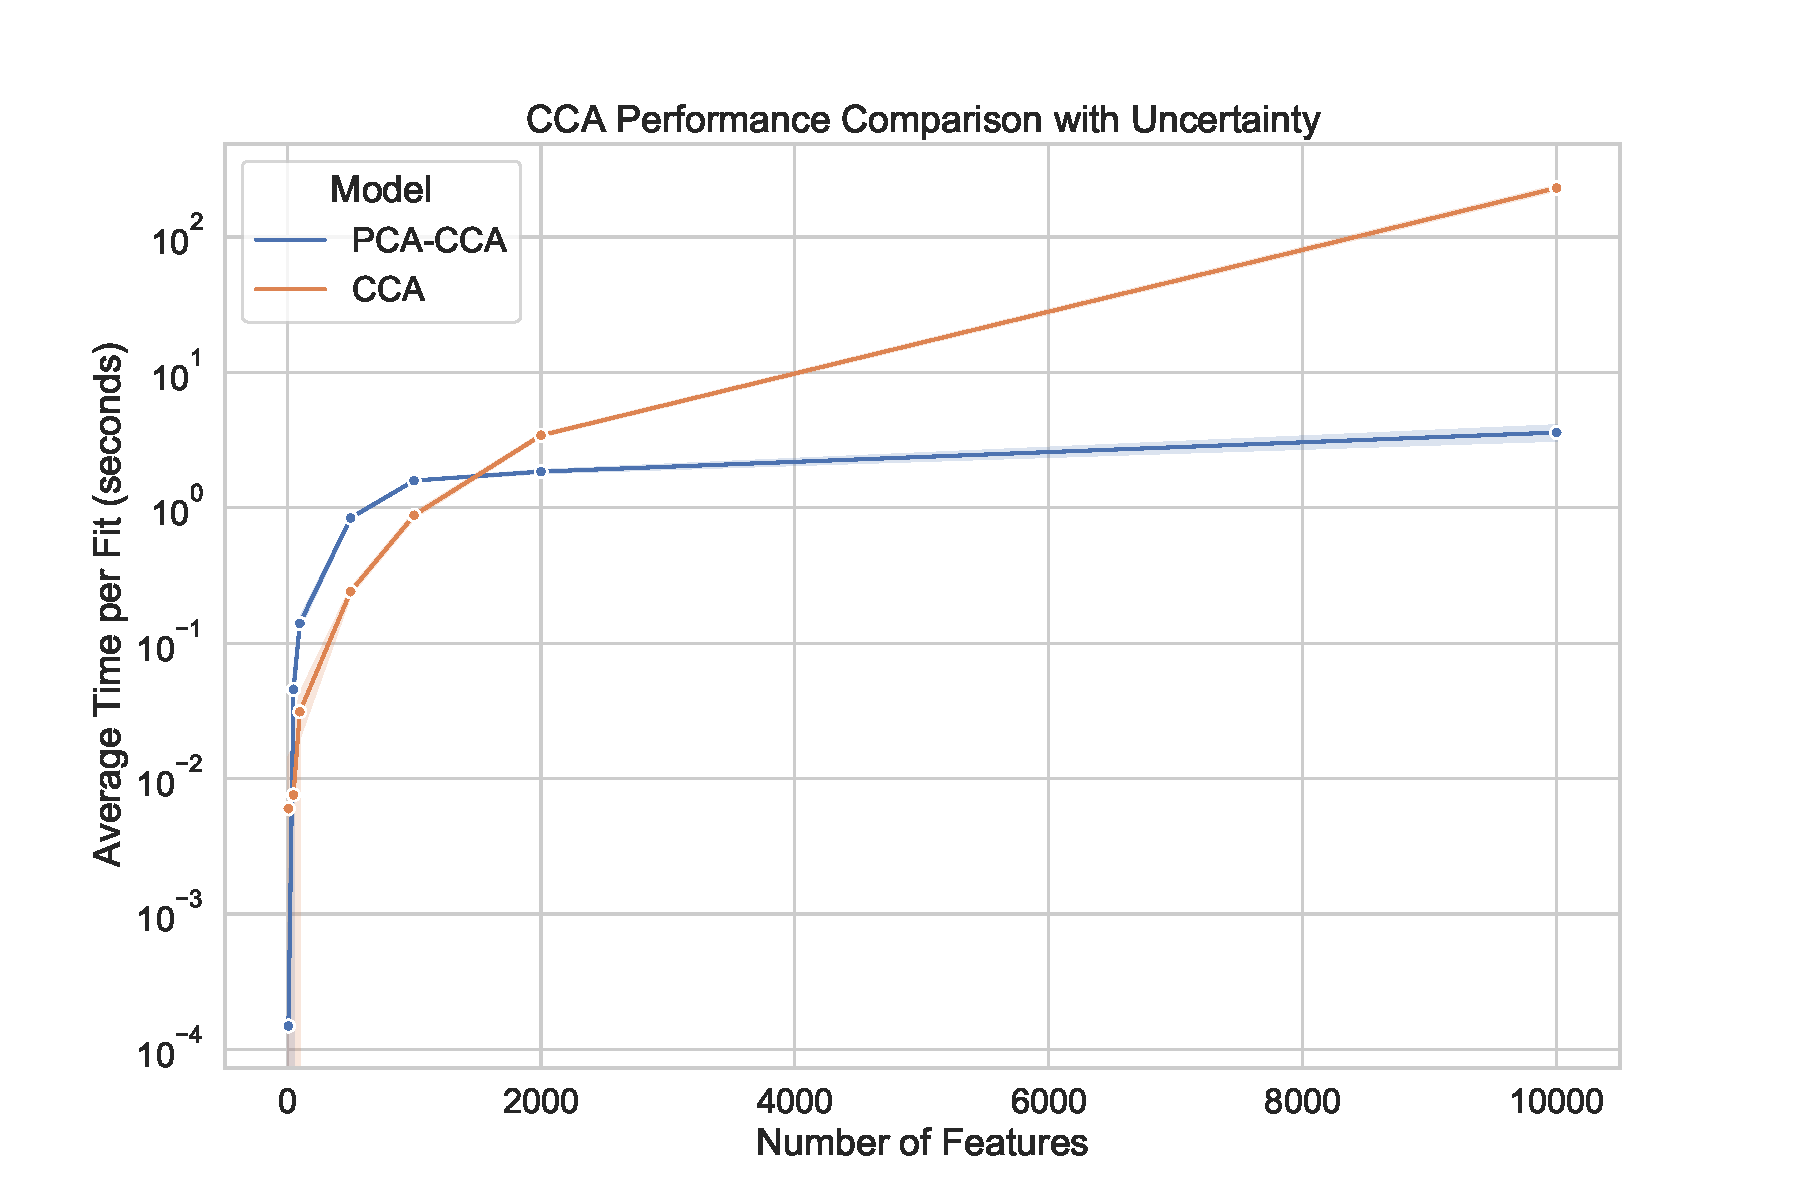
\includegraphics[width=0.7\textwidth]{figures/benchmarks/ccapca_comparison_log}
     \caption{Comparison of the complexity of PCA-CCA and CCA for varying numbers of samples and features.}
     \label{fig:pca-cca-complexity}
 \end{figure}

This approach has been employed to great effect in neuroimaging but suprisingly is not used even in the scikit-learn implementation of \acrshort{cca} \citep{pedregosa2011scikit}.
Nonetheless, for the large sample sizes (desirable for machine learning frameworks as well as statistical power), the complexity of even \acrshort{pca}-CCA can render the problems nearly intractable.

\subsubsection{Kernel CCA}

Kernel \acrshort{cca} (\acrshort{kcca}) also offers computational efficiency for high-dimensional data (\(p_i>n\)) as its complexity scales with the number of samples \(n\), not the number of features \(p_i\)\citep{akaho2006kernel}.
It casts the CCA optimisation as a dual problem:

\begin{align}
    & \alpha_{\text{opt}}=\underset{\alpha}{\mathrm{argmax}}\{ \alpha\sps{1}K\spsT{1}K\sps{2}\alpha\sps{2}  \} \\
    & \text{subject to:} \notag                                                                                            \\
    & \alpha\sps{1}K\spsT{1}K\sps{1}\alpha\sps{1}=1 \notag                                                                  \\
    & \alpha\sps{2}K\spsT{2}K\sps{2}\alpha\sps{2}=1 \notag
\end{align}

Where \(\alpha\sps{i}=\) are dual variables, \(K\sps{i}\) are kernel matrices, and \(K\spsT{i}\) are their transposes.
The kernel matrices are defined as \(K\sps{i}=\phi(X\sps{i})\phi(X\sps{i})^T\), where \(\phi(\cdot)\) is a nonlinear mapping function.
The kernel trick is used to avoid the explicit computation of the nonlinear mapping function \(\phi(\cdot)\).
The complexity of \acrshort{kcca} is \(\mathcal{O}(n^3)\), which can be much lower than the complexity of solving the original GEP directly when \(p_i>n\).
However, a significant drawback of KCCA is the need for access to all training data at test time, which raises concerns about efficiency and scalability.
Furthermore, when the number of samples is large, the kernel matrix can itself be too large to fit in memory.

\subsection{Stochastic Algorithms for CCA}

\subsubsection{Classical Iterative Algorithms for PCA}
In order to gain the intuition behind a number of stochastic algorithms for CCA, it's essential to understand the classical iterative algorithms for generalized eigenvalue problems, such as Sanger's rule \cite{sanger1989optimal} (the generalized Hebbian algorithm (GHA)) and Oja's rule.

The power method is a simple iterative algorithm for finding the dominant eigenvector of a matrix $A$. The update rule for the power method is:
\begin{align}
u \leftarrow \frac{A u}{\|A u\|}
\end{align}
where $u$ is the current estimate of the dominant eigenvector. The power method converges to the dominant eigenvector of $A$ under mild conditions.

Sanger's rule \citep{sanger1989optimal}, also known as the GHA, is an iterative learning rule for finding the principal components of a data set. It can be written as:
\begin{align}
U \leftarrow U + \eta \left( A U - U \text{tril}(U^T A U) \right)
\end{align}
where \( \text{tril}(\cdot) \) denotes the lower triangular part of a matrix.

Oja's rule \citep{oja1982simplified}, a simplified version of Sanger's rule, can be written as:
\begin{align}
U \leftarrow U + \eta \left( A U - U (U^T A U) \right)
\end{align}

In order to maintain orthogonality of the eigenvectors during the iterative updates, Oja's rule can be combined with a QR decomposition step:
\begin{align}
U \leftarrow U + \eta \left( A U - U (U^T A U) \right) \\
U \leftarrow \text{qr}(U)
\end{align}
where \( \text{qr}(\cdot) \) denotes the QR decomposition, which factorizes a matrix into an orthogonal matrix $Q$ and an upper triangular matrix $R$. By using only the orthogonal matrix $Q$, we ensure that the eigenvectors remain orthogonal throughout the iterative process. Alternatively, other orthogonalization techniques such as Gram-Schmidt process \citep{schmidt1907theorie,wong1935application} can be employed.

Both Sanger's rule and Oja's rule aim to find the principal subspace of a matrix \( A \), which is equivalent to solving the eigenvalue problem \( A U = U \Lambda \) where \( \Lambda \) is a diagonal matrix of eigenvalues. These algorithms can be seen as iterative methods for solving the optimization problem:
\begin{align}
\max_{U} \Tr \left(U^T A U\right) \quad \text{subject to} \quad U^T U = I
\end{align}

GHA can also be extended to solve the generalized eigenvalue problem $A U = B U \Lambda$, where $B$ is a positive definite matrix\citep{chen2019constrained}. The update rule for this problem is:
\begin{align}
U \leftarrow U + \eta \left( A U - B U \text{tril}(U^T A U) \right)
\end{align}
which subsumes the original GHA as a special case when $B=I$.

A number of algorithms have been proposed to approximate GEPs including PCA and PLS \citep{arora2012stochastic}, and CCA specifically \citep{bhatia2018gen}, in the `stochastic' or `data-streaming' setting; these can have big computational savings.

\subsection{Stochastic Power Method}
\citet{arora2016stochastic} demonstrate that PLS can be approximated by applying a stochastic Power Method. For PLS, the iterations are computed by:
\begin{align*}
U^{(1)}t &= \mathcal{P}{\text{orth}} \left( U^{(1)}{t-1} + \eta_t X_t Y_t^\top U^{(2)}{t-1} \right), \\
U^{(2)}t &= \mathcal{P}{\text{orth}} \left( U^{(2)}{t-1} + \eta_t Y_t X_t^\top U^{(1)}{t-1} \right),
\end{align*}
where \( \mathcal{P}_{\text{orth}}(\cdot) \) represents an orthogonal projection operator that projects a vector or matrix onto the space orthogonal to the current subspace. \( \hat{U}^{(1)}_t \) and \( \hat{U}^{(2)}_t \) are the current estimates of the left and right singular vectors for the two views, \( X_t \) and \( Y_t \) are the new data points at time \( t \), and \( \eta_t \) is the learning rate at time \( t \).
The approach has low computational complexity, $\mathcal{O}(k(p_1+ p_2))$.
However, there are two main drawbacks to this approach.
First, convergence is not guaranteed.
Second, the orthogonal projection step does not extend naturally to the CCA problem where the constraint is \( U^\top B U = I \) rather than \( U^\top U = I \).

\subsubsection{SGHA}
SGHA is an algorithm for finding the top-k generalized eigenvectors of a matrix pair ( (A, B) ), where \( A \) is symmetric and \( B \) is symmetric positive definite. It builds upon the generalized Hebbian algorithm (GHA).
Specifically, they form the constrained optimization problem for the top-k subspace as:
\begin{align}
\min_{U} -\Tr \left(U^T A U\right) \quad \text{subject to} \quad U^T B U = I
\end{align}
Transforming this into an unconstrained problem using Lagrange multipliers:
\begin{align}
\min_{U} -\Tr\left(U^T A U \right) + \lambda \left(U^T B U - I\right)
\end{align}
Differentiating with respect to \( U \) and \( \lambda \) gives the stationary points:
\begin{align}
2 A U - 2 B U \lambda = 0 \quad \text{and} \quad U^T B U - I = 0\\
\implies \lambda = U^T A U
\end{align}

Given this, the authors propose a primal dual update rule:
\begin{align}
U \leftarrow U - \eta \left( A U - B U \lambda \right)
\lambda \leftarrow \left( U^T A U \right)
\end{align}
where \( \eta \) is a learning rate.

These updates can also be combined into a single update rule:
\begin{align}
U \leftarrow U - \eta \left( A U - B U \left( U^T A U \right) \right)
\end{align}

This algorithm is very simple to implement but because it is based on a heuristic primal-dual update rule rather than gradient descent, it is hard to use with more sophisticated optimizers such as Adam \citep{kingma2014adam}.

\subsubsection{$\gamma$-EigenGame}
The $\gamma$-EigenGame is a stochastic algorithm for CCA inspired by the $\gamma$-EigenGame algorithm for PCA. The key idea behind the EigenGame algorithms is to view the eigenvectors as competing players trying to explain the data. In this game-theoretic perspective, each eigenvector (player) $u_i$ aims to maximize its own utility function:
\begin{align}
\max_{u_i} \overbrace{\frac{u_i^TAu_i}{u_i^TBu_i}}^{\text{rewards}} - \overbrace{\sum_{j < i} \frac{(u_j^TAu_j)(u_i^TBu_j)^2}{(u_j^TBu_j)^2(u_i^TBu_i)}}^{\text{penalties}}
\end{align}
The utility function consists of a reward term, $\frac{u_i^TAu_i}{u_i^TBu_i}$, which encourages the eigenvector to align with the direction of maximum variance in the data, and a penalty term, $\sum_{j < i} \frac{(u_j^TAu_j)(u_i^TBu_j)^2}{(u_j^TBu_j)^2(u_i^TBu_i)}$, which discourages the eigenvector from aligning with the directions already captured by the previous eigenvectors.

A key advantage of the $\gamma$-EigenGame formulation is that each player $i$ only needs to maintain orthogonalization with respect to the previous players $j < i$. This allows for a more efficient and decentralized computation of the eigenvectors.

By applying a few heuristic arguments, the $\gamma$-EigenGame algorithm derives an update rule for each eigenvector in the full batch case:
\begin{align}
u_i \leftarrow (u_i^T B u_i)A u_i - (u_i^T A u_i)B u_i - \sum_{j < i} (u_i^T A y_j)[(u_i^T B u_i)B y_j - (u_i^T B y_j)B u_i]
\end{align}
where $y_j = \frac{u_j}{\sqrt{u_j^TBu_j}}$. This update rule adjusts the eigenvector $u_i$ to maximize its utility, considering the rewards and penalties.

In the stochastic version of the $\gamma$-EigenGame algorithm, the update rule is modified to use a rolling average of the matrix $B$, introducing an additional hyperparameter $\gamma$ that needs to be tuned. This stochastic update helps to reduce the computational complexity and memory requirements of the algorithm, making it more suitable for large-scale problems.

To the best of our knowledge, the state-of-the-art in Stochastic PLS and CCA are the subspace Generalized Hebbian Algorithm (SGHA) \citep{chen2019constrained} and $\gamma$-EigenGame \citep{gemp20,gemp2021}.

\subsubsection{Further Benefits of Stochastic Algorithms}
Stochastic algorithms not only offer computational advantages but also introduce a form of implicit regularization \citep{smith2021origin}, which can be particularly beneficial in high-dimensional settings. Regularization techniques are commonly used to prevent overfitting and improve the generalization performance of models, especially when dealing with limited data or complex models.

As we have seen, in batch learning algorithms, regularization is often explicit, such as adding L1 or L2 penalty terms to the objective function. These penalty terms constrain the model's parameters and discourage overfitting. However, stochastic algorithms inherently introduce regularization through the noise in the stochastic updates, without the need for explicit penalty terms.

The intuition behind the regularizing effect of stochastic algorithms can be understood as follows:

\begin{itemize}
    \item \textbf{Stochastic updates introduce noise}: In each iteration of a stochastic algorithm, the update is based on a random subset of the data (a mini-batch) rather than the entire dataset. This introduces noise in the updates, causing the model's parameters to fluctuate around their true values. The noise can be seen as a form of random perturbation that helps the algorithm explore the parameter space and escape from shallow local minima.
    \item \textbf{Noisy updates prevent overfitting}: The noise in the stochastic updates acts as a form of regularization that prevents the model from fitting too closely to the training data. By introducing this randomness, stochastic algorithms reduce the risk of overfitting, especially when the model has a large number of parameters relative to the size of the training data. The noisy updates effectively smooth out the loss function, making it harder for the model to memorize individual training examples.

    \item \textbf{Averaging effect}: As the stochastic algorithm progresses, the noisy updates tend to cancel out each other over time, leading to an averaging effect. This averaging helps the model converge towards a solution that generalizes well to unseen data, rather than getting stuck in a suboptimal solution that overfits the training data. Intuitively, the averaging effect can be seen as a form of ensembling, where multiple noisy models are combined to produce a more robust and generalizable solution.
    
    \item \textbf{Implicit bias towards simpler models}: The noise in the stochastic updates implicitly biases the algorithm towards simpler models that are less prone to overfitting. This is because simpler models are more stable under random perturbations, while complex models that overfit the data are more sensitive to noise. As a result, stochastic algorithms tend to favor models with smoother decision boundaries and better generalization performance, even without explicit regularization terms in the objective function.
\end{itemize}

The regularizing effect of stochastic algorithms has been extensively studied in the context of deep learning \citep{zhang2021understanding,chaudhari2018stochastic}. These studies have shown that the implicit regularization introduced by stochastic updates can lead to improved generalization performance and robustness to noise, especially in high-dimensional settings where the number of parameters is large compared to the number of training examples.

\subsection{Limitations of Existing Stochastic CCA Algorithms}
While stochastic algorithms like SGHA and $\gamma$-EigenGame have made significant progress in addressing the computational challenges of CCA in high-dimensional settings, they still have some limitations that motivate the development of novel objectives and algorithms.

One limitation of SGHA is that it relies on a heuristic primal-dual update rule rather than a principled optimization framework. This makes it difficult to integrate with more sophisticated optimizers like Adam \citep{kingma2014adam}, which have been shown to improve convergence speed and stability in many machine learning applications.

On the other hand, $\gamma$-EigenGame requires the tuning of a hyperparameter $\gamma$ in the stochastic setting. This hyperparameter controls the trade-off between the computational efficiency and the accuracy of the stochastic updates, and its optimal value may vary depending on the problem and the data.

To address the limitations of existing stochastic CCA algorithms and provide a more principled and robust approach, we propose a novel formulation of the CCA problem based on the Eckhart--Young--Minsky inequality \citep{stewart_matrix_1990}. Our formulation leads to a new objective function that characterizes the top-$K$ subspace of Generalized Eigenvalue Problems (GEPs), including CCA as a special case.

\section{Methods: Novel Objectives and Algorithms}\label{sec:contributions}

First, we present proposition \ref{prop:EY-charac}, a formulation of the top-$K$ subspace of GEP problems, which follows by applying the Eckhart--Young--Minsky inequality \citep{stewart_matrix_1990} to the eigen-decomposition of $B^\mhalf A B^\mhalf$. However, making this rigorous requires some technical care which we defer to the proof in supplement \ref{app:gradient_descent}\ref{supp:proofs}.   

\begin{restatable}[Eckhart--Young inspired objective for GEPs]{proposition}{EYcharac}
\label{prop:EY-charac}
    The top-$K$ subspace of the GEP $(A,B)$ can be characterized by minimizing the following objective over $U \in \R^{D \times K}$:
    \begin{align}\label{eq:EY-charac}
        \LEYGEP(U) \defeq \tr \left( - 2\,U^\top A U + \left(U^\top B U\right) \left(U^\top B U\right) \right)
    \end{align}
    Moreover, the minimum value is precisely $- \sum_{k=1}^K \lambda_k^2$, where $(\lambda_k)$ are the generalized eigenvalues.
\end{restatable}

The objective in Equation \eqref{eq:EY-charac} has an intuitive interpretation. The first term, $-2 \tr(U^\top A U)$, acts as a reward for high covariance between the views, encouraging the learned subspace to capture the directions of maximum correlation. The second term, $\tr((U^\top B U)(U^\top B U))$, serves as a penalty for high variance within each view and promotes orthogonality between the learned components. By minimizing this objective, we aim to find a subspace that maximizes the correlation between views while ensuring the learned components are distinct and informative.

This objective also has appealing geometrical properties. 
It is closely related to a wide class of unconstrained objectives for PCA and matrix completion which have no spurious local optima \citep{ge_no_2017}, i.e. all local optima are in fact global optima. 
This implies that certain local search algorithms, such as stochastic gradient descent, should indeed converge to a global optimum.

\begin{restatable}{proposition}{NoSpuriousLocalMinima}\label{prop:no-spurious}
    The objective $\LEYGEP$ has no spurious local minima.
    That is, any matrix $\bar{U}$ that is a local minimum of $\LEYGEP$ must in fact be a global minimum.
    %of the form described in \cref{prop:EY-charac}
\end{restatable}

It is also possible to make this argument quantitative by proving a version of the strict saddle property from \citet{ge_no_2017,ge2015escaping}; we state an informal version here and give full details in \ref{app:gradient_descent}\ref{supp:tractable-optimization}.

\begin{corollary}[Informal: Polynomial-time Optimization]
    Under certain conditions on the eigenvalues and generalized eigenvalues of $(A,B)$, one can make quantitative the claim that:
    any $U_K \in \R^{D \times K}$ is either close to a global optimum, has a large gradient $\nabla \LEYGEP$, or has Hessian $\nabla^2 \LEYGEP$ with a large negative eigenvalue.
    
    Therefore, for appropriate step-size sequences, certain local search algorithms, such as sufficiently noisy SGD, will converge in polynomial time with high probability.
    % still need to sort out - polynomial in what exactly!
\end{corollary}

\subsection{Corresponding Objectives for the CCA family}
For the case of linear CCA we have $U^\top A U = \sum_{i \neq j} \Cov(Z\sps{i}, Z\sps{j}),\,  U^\top B U = \sum_{i} \Var(Z\sps{i})$. 

To generalize this to multiview CCA, we define the analogous matrices of total between-view covariance and total within-view variance 
\begin{align}\label{eq:def-C-V-matrices}
    \vphantom{\bigl(\bigr)} % increase vertical space
    C(\theta) = \sum_{i \neq j} \Cov(Z\sps{i}, Z\sps{j}), \quad 
    V(\theta) = \sum_{i} \Var(Z\sps{i})
\end{align}

While for ridge CCA we can add a ridge penalty to the within-view variances:
\begin{align}\label{eq:v-alpha-ridge-definition}
    V_\alpha(\theta) = \sum_i \alpha_i {U\spsT{i}} U\sps{i} +  (1 - \alpha_i) \Var(Z\sps{i})
\end{align}
This leads to the following unconstrained objective for the CCA-family of problems.
\begin{definition}[Family of EY Objectives]\ref{def:EY-objectives}
    Learn representations $Z\sps{i} = f\sps{i}( X\sps{i}; \theta\sps{i})$ minimizing
    \begin{align}\label{eq:EY-loss-def-C-V}
        \LEY(\theta) = - 2 \tr C(\theta) + \norm{V_\alpha(\theta)}_F^2
    \end{align}
\end{definition}

\textbf{Unbiased estimates:}
since empirical covariance matrices are unbiased, we can construct unbiased estimates to $C, V$ from a batch of transformed variables $\Z$.
\begin{align}\label{eq:def-C-V-matrices-empirical}
    \hat{C}(\theta)[\Z] = \sum_{i \neq j} \empCov(\Z\sps{i}, \Z\sps{j}), \quad 
    \hat{V}(\theta)[\Z] = \sum_{i} \empVar(\Z\sps{i})
\end{align}
In the linear case we can construct $\hat{V}_\alpha(\theta)[\Z]$ analogously by plugging sample covariances into \cref{eq:v-alpha-ridge-definition}.
Then if $\Z, \Z'$ are two independent batches of transformed variables, the batch loss
\begin{align}\label{eq:empirical-EY-loss-estimate-def}
    \empLEY[\Z, \Z'] \defeq - 2 \tr \hat{C}[\Z] + \langle \hat{V}_\alpha[\Z], \hat{V}_\alpha[\Z'] \rangle_F
\end{align}
gives an unbiased estimate of $\LEY(\theta)$.%\footnote{Where again $\alpha > 0$ only makes sense in the linear case, and otherwise we may omit the $\alpha$s}
This loss is a differentiable function of $\Z, \Z'$ and so also of $\theta$.

\textbf{Simple algorithms:}
We first define a general algorithm using these estimates in Algorithm \ref{alg:general}. In the next section we apply this algorithm to multiview stochastic CCA (\textbf{CCA-EY}) and PLS (\textbf{PLS-EY}).

\begin{algorithm}
   \caption{\textbf{GEP-EY}: General algorithm for learning correlated representations}
   \label{alg:general}
\begin{algorithmic}
   \STATE {\bfseries Input:} data stream of mini-batches $(\X(b))_{b=1}^\infty$ where each consists of $M$ samples from the original dataset. Learning rate $(\eta_t)_t$. Number of time steps $T$. Class of functions $f(\cdot; \theta)$ whose outputs are differentiable with respect to $\theta$.
   \STATE {\bfseries Initialize:} $\hat{\theta}$ with suitably random entries
   \FOR{$t=1$ {\bfseries to} $T$}
       \STATE Obtain two independent mini-batches \( \X(b), \X(b') \) by sampling \( b, b' \) independently
       \STATE Compute batches of transformed variables $\Z(b) = f(\X(b); \theta), \Z(b') = f(\X(b'); \theta)$
       %\STATE Construct unbiased estimates $C(\theta)[\Z], \hat{V}(\theta)[\Z], \hat{V}(\theta)[\Z']$ \COMMENT{As defined in \cref{eq:def-C-V-matrices-empirical}}
       \STATE Estimate loss $\empLEY(\theta)$ using \cref{eq:empirical-EY-loss-estimate-def}
       \STATE Obtain gradients by back-propagation and step with your favourite optimizer.
   \ENDFOR
\end{algorithmic}
\end{algorithm}

\subsection{Applications to multiview stochastic CCA and PLS}
\begin{lemma}[Objective recovers GEP formulation of linear multiview CCA]
    When the $f\sps{i}$ are linear, the population loss from \cref{eq:EY-loss-def-C-V} recovers MCCA.
\end{lemma}
\begin{proof}
    By construction, for linear MCCA we have $C = U^\top A U,\, V_\alpha=U^\top B_\alpha U$, where $(A, B_\alpha)$ define the GEP for MCCA introduced in \cref{eq:gep-most-general-formulation}. 
    So $\LEY(U) = \LEYGEP(U)$ and by \cref{prop:EY-charac} the optimal set of weights define a top-$K$ subspace of the GEP, and so is a MCCA solution.
    %; by definition, $\MCCA_K$ is the vector of top-$K$ generalised eigenvalues, so the optimal value is as claimed.
\end{proof}

Moreover, by following through the chain of back-propagation, we obtain gradient estimates in $\mathcal{O}(MKD)$ time.
Indeed, we can obtain gradients for the transformed variables in $\mathcal{O}(M K^2)$ time so the dominant cost is then updating $U$; we flesh this out with full details in \cref{supp:fast-updates}.

\section{Experiments and Results}

\subsection{Comparison to Scipy}
In a first simple experiment, we compare our method to solving the CCA Generalized Eigenvalue Problem using the \texttt{scipy} implementation of \texttt{eigh} \citep{virtanen2020scipy}.
We use a sample size of 10,000 and vary the number of features in each view from 10 to 5,000.
We solve for the top-5 CCA subspace and repeat each experiment 5 times.
We compare the time taken to solve the GEP using \texttt{eigh} to the time taken to train our method until the frobenius norm of the change in successive weights is less than $10^{-5}$.

\subsubsection{Observations}
Figure \ref{fig:cca-comparison} shows the results of this experiment.
Up until 1,000 features, our method is slower than \texttt{eigh} but after this point, our method is significantly faster.
Beyond this point, the time taken to solve the GEP using \texttt{eigh} scales quadratically with the number of features, while our method scales linearly.
This is because our method scales linearly with both the number of samples and the number of features, while \texttt{eigh} scales quadratically with the number of features\footnote{When the number of features is greater than the number of samples as in ridge CCA and PLS, we can use the PCA or Kernel trikcs to scale CCA quadratically with the minimum of the number of features and samples, though this still requires a somewhat expensive PCA}.

\begin{figure}
    \centering
    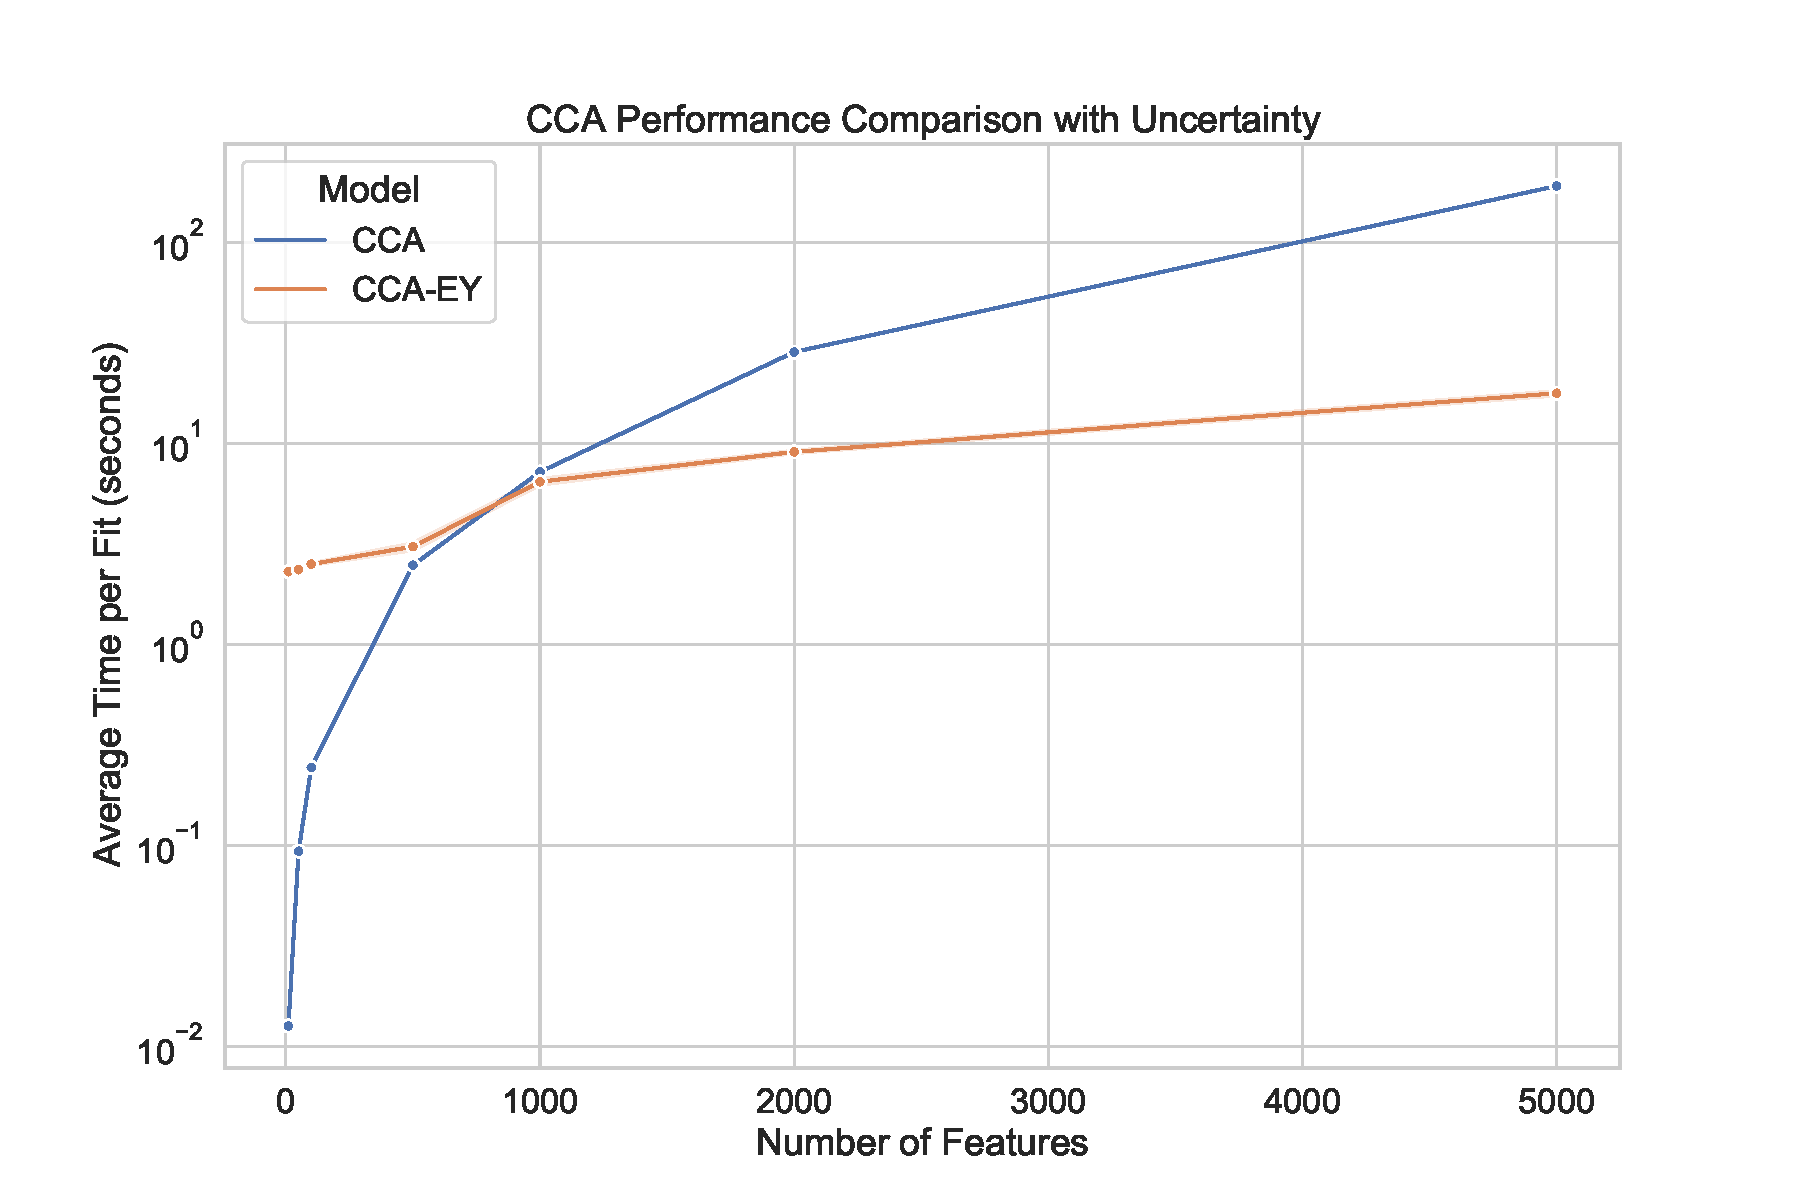
\includegraphics[width=0.8\textwidth]{figures/benchmarks/cca_comparison_log}
    \caption{Comparison of the time taken to solve CCA using \texttt{eigh} and our CCA-EY method.}
    \label{fig:cca-comparison}
\end{figure}

\subsection{Stochastic CCA}
In our second experiment, we aim to demonstrate that our proposed CCA-EY method not only matches but potentially surpasses the performance of established baselines $\gamma$-EigenGame and SGHA in terms of convergence speed and robustness to hyperparameter settings.
Our experimental setup largely follows the framework established by \citet{meng2021online, gemp2022generalized}.
A key distinction in our approach, however, is the decision to not perform PCA on the data prior to applying CCA methods.
This choice retains the full complexity of the datasets, providing a more rigorous evaluation of each algorithm's ability to handle high-dimensional data efficiently and accurately.

One of the central goals of this comparison is to illustrate that CCA-EY can achieve faster convergence with less hyperparameter tuning, an essential attribute for practical applications.
To facilitate a fair and direct comparison with the baseline methods, we employ Stochastic Gradient Descent (SGD) as the optimization technique for all algorithms.
It is worth noting that while SGD provides a baseline for performance assessment, the potential of our CCA-EY method could be further unleashed by utilizing more advanced optimization techniques such as momentum-based optimizers like Adam or Nesterov acceleration.
These advanced methods are known for their ability to accelerate convergence and navigate the optimization landscape more effectively, suggesting that our method might yield even better performance under such enhanced optimization schemes.

We train models to optimize CCA on the MediaMill and Split-CIFAR-10 datasets for a single epoch, using mini-batch sizes ranging from 5 to 100.
These sizes were selected to test the scalability and efficiency of our method under varied computational loads. The Proportion of Correlation Captured (PCC) metric, defined as \( \text{PCC} = (\sum_{i=k}^K \rho_k)/ ({\sum_{k=1}^K \rho_k^*}) \), serves as our evaluation criterion.
Here, $\rho_k$ represents the correlations of the estimated representations $Z\sps{i}=X^{(i)}\hat{U}^{(i)}$ with one another on the test set, while $\rho_k^*$ denotes the canonical correlations computed from the full batch covariance matrices.
In other words, using our earlier notation, $\rho_k = \MCCA_K(\hat{Z}\sps{1}, \hat{Z}\sps{2})$ and $\rho_k^* = \MCCA_K(X\sps{1}, X\sps{2})$.

Despite $\rho_k^*$ not being the `true` correlations, their computation from a large sample size renders them a reliable benchmark.
PCC is an efficient metric for tracking algorithmic performance over time, minimizing computational overhead\citep{meng2021online, gemp2022generalized, ma2015finding, ge2016efficient}.

\subsubsection{Data}
The MediaMill dataset \citep{gemert2008visual} comprises paired features of videos and corresponding commentary, with the objective of learning joint representations that capture their correlation.
This representation could potentially enable prediction of commentary from video, or vice versa.
The dataset includes 25,800 test images, with 120 and 101 features respectively.

The Split-CIFAR dataset \citep{meng2021online} consists of 50,000 training and 10,000 test RGB images, each split in half with 32x16x3 features.
The aim is to learn joint representations of the two halves that reveal correlations, expected to be high within the same class and low across different classes.
These datasets are chosen for their diverse nature and complexity, providing a comprehensive test bed for our method.

\subsubsection{Parameters} For each method, we searched over the hyperparameter (see Table \ref{tab:hyperparameters}) using \citet{wandb}.

\begin{table}[h!]
    \centering
    \begin{tabular}{|l|l|}
        \hline Parameter             & Values              \\
        \hline minibatch size        & 5,20,50,100         \\
        \hline components            & 5                   \\
        \hline epochs                & 1                   \\
        \hline seed                  & 1, 2, 3, 4, 5       \\
        \hline lr                    & 0.01, 0.001, 0.0001 \\
        \hline $\gamma$\footnote{gamma is only used for $\gamma$-EigenGame} & 0.01,0.1,1,10       \\
        \hline
    \end{tabular}
    \caption{Hyperparameter ranges explored for CCA methods.} 
    \label{tab:hyperparameters}
\end{table}

\subsubsection{Observations}
In machine learning, a learning curve represents a graph showing the model's learning progress over time in terms of experience or iterations.
For the MediaMill dataset, Figure \ref{fig:corr_mediamill} compares the algorithms' learning curves for various mini-batch sizes, showing CCA-EY's consistent outperformance. Figure \ref{fig:learningcurve_mediamill} further examines the learning curves for batch sizes 5 and 100, illustrating CCA-EY's superior performance over time.

\begin{figure}
    \centering
    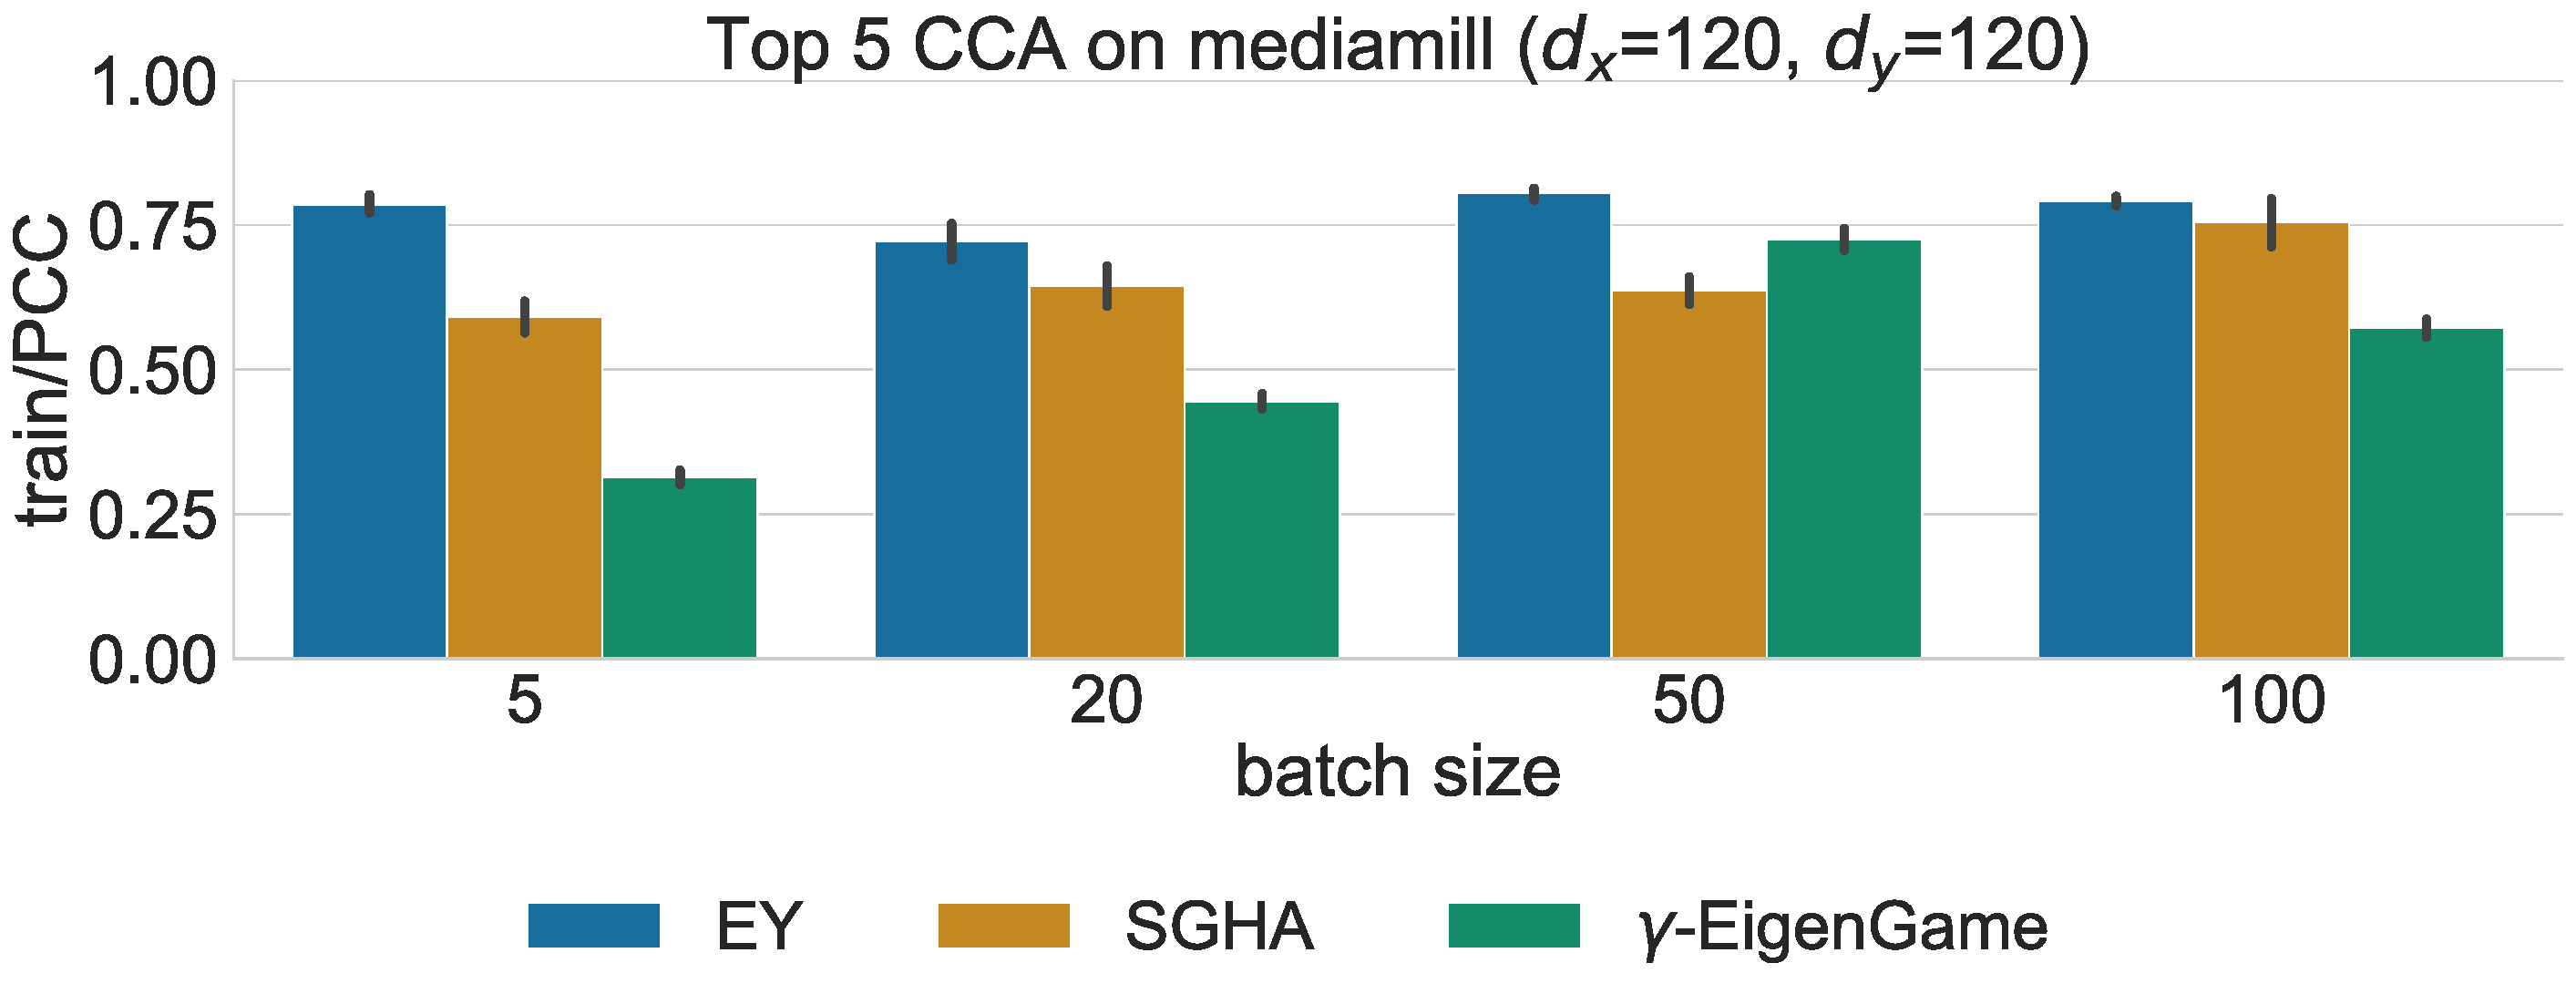
\includegraphics[width=0.8\textwidth]{figures/CCA/mediamill_models_different_batch_sizes}
    \caption{Stochastic CCA on MediaMill using PCC: Performance across varying mini-batch sizes. Shaded regions signify \(\pm\) one standard deviation around the mean of 5 runs.}
    \label{fig:corr_mediamill}
\end{figure}

\begin{figure}
    \centering
    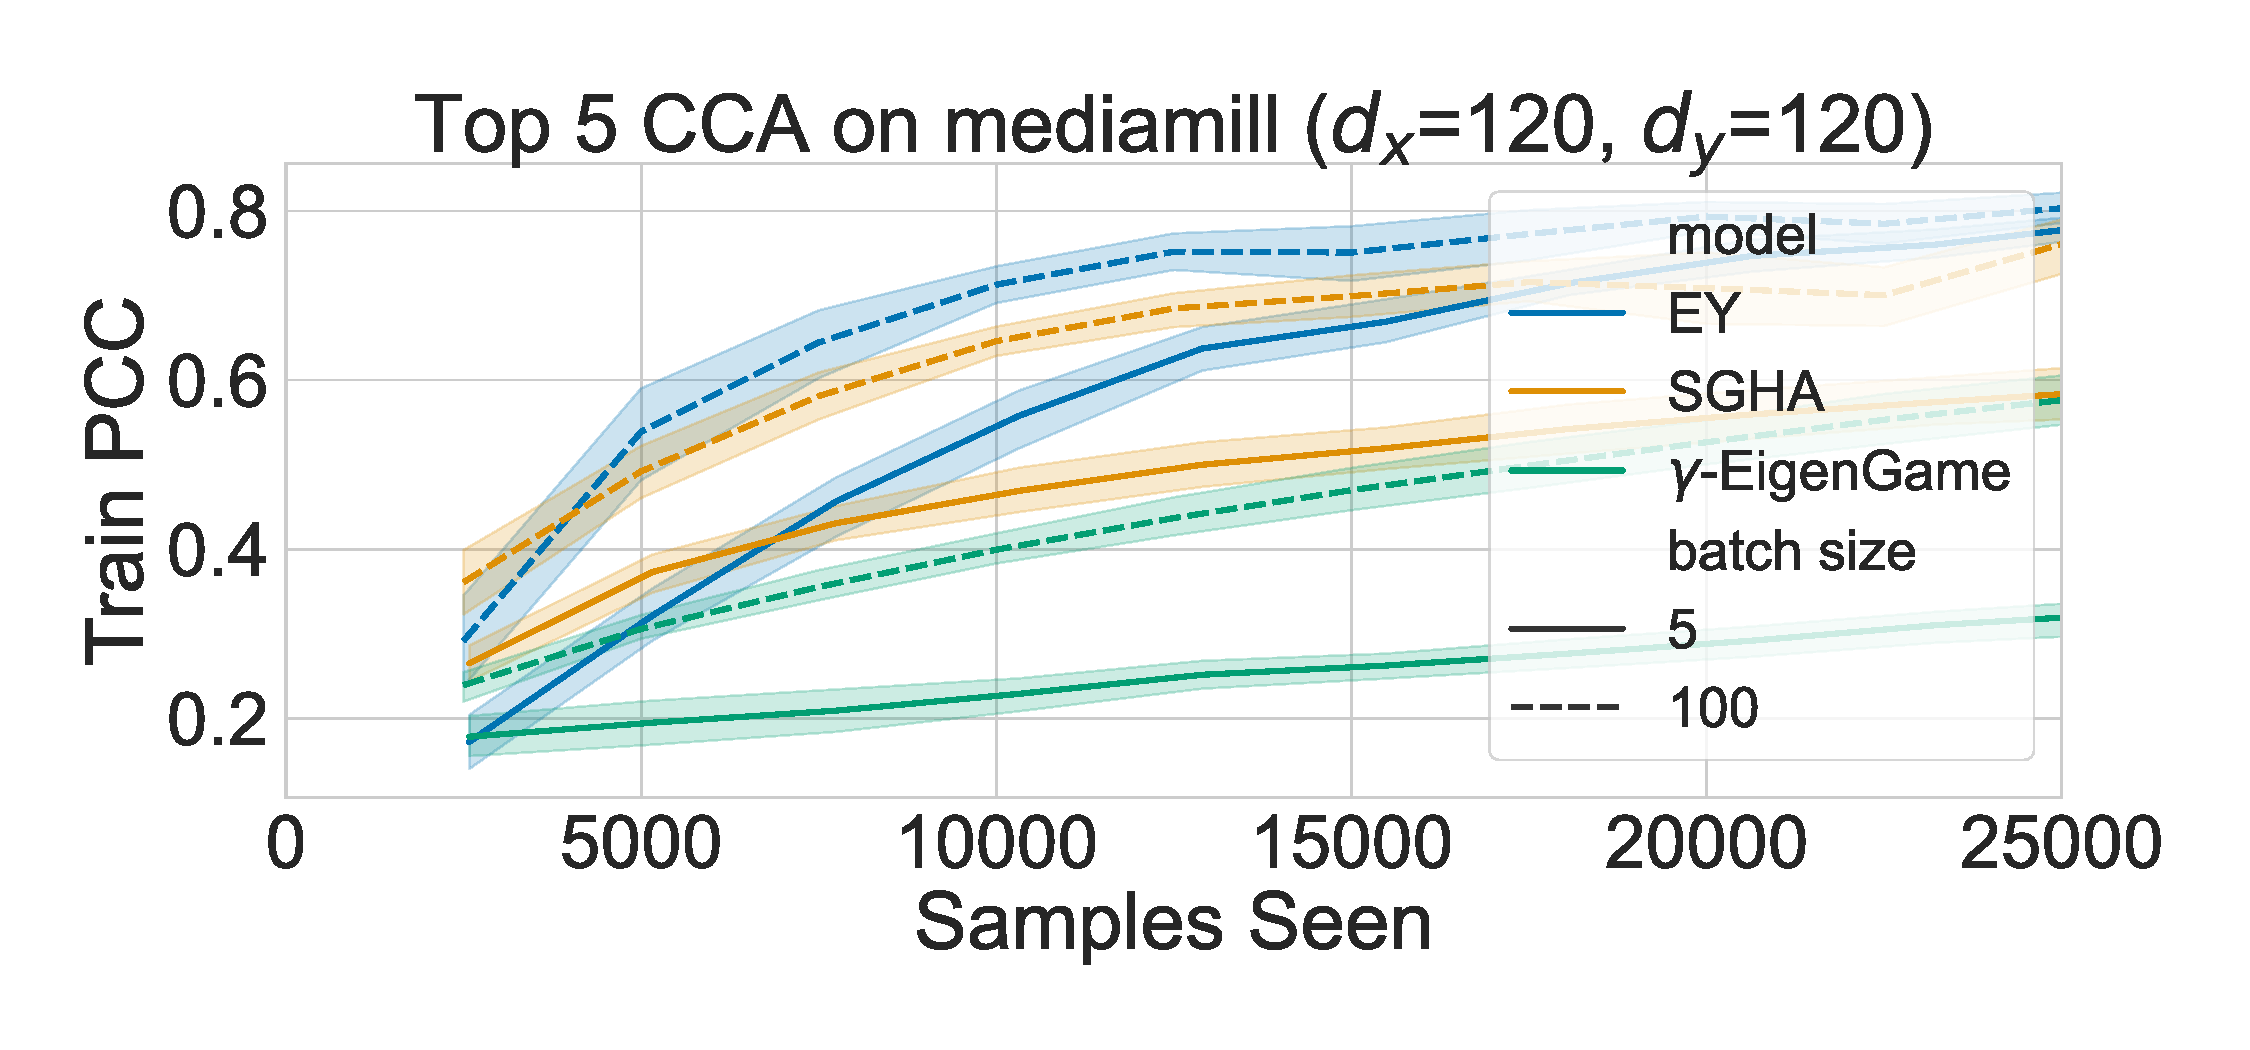
\includegraphics[width=0.8\textwidth]{figures/CCA/mediamill_allbatchsizes_pcc}
    \caption{Stochastic CCA on MediaMill: Training progress over a single epoch for mini-batch sizes 5, 100.}
    \label{fig:learningcurve_mediamill}
\end{figure}

For the CIFAR dataset, Figure \ref{fig:corr_cifar} shows the performance comparison across batch sizes, while Figure \ref{fig:learningcurve_cifar} details the learning curves, highlighting the underperformance of $\gamma$-EigenGame, especially for smaller batch sizes.

\begin{figure}
    \centering
    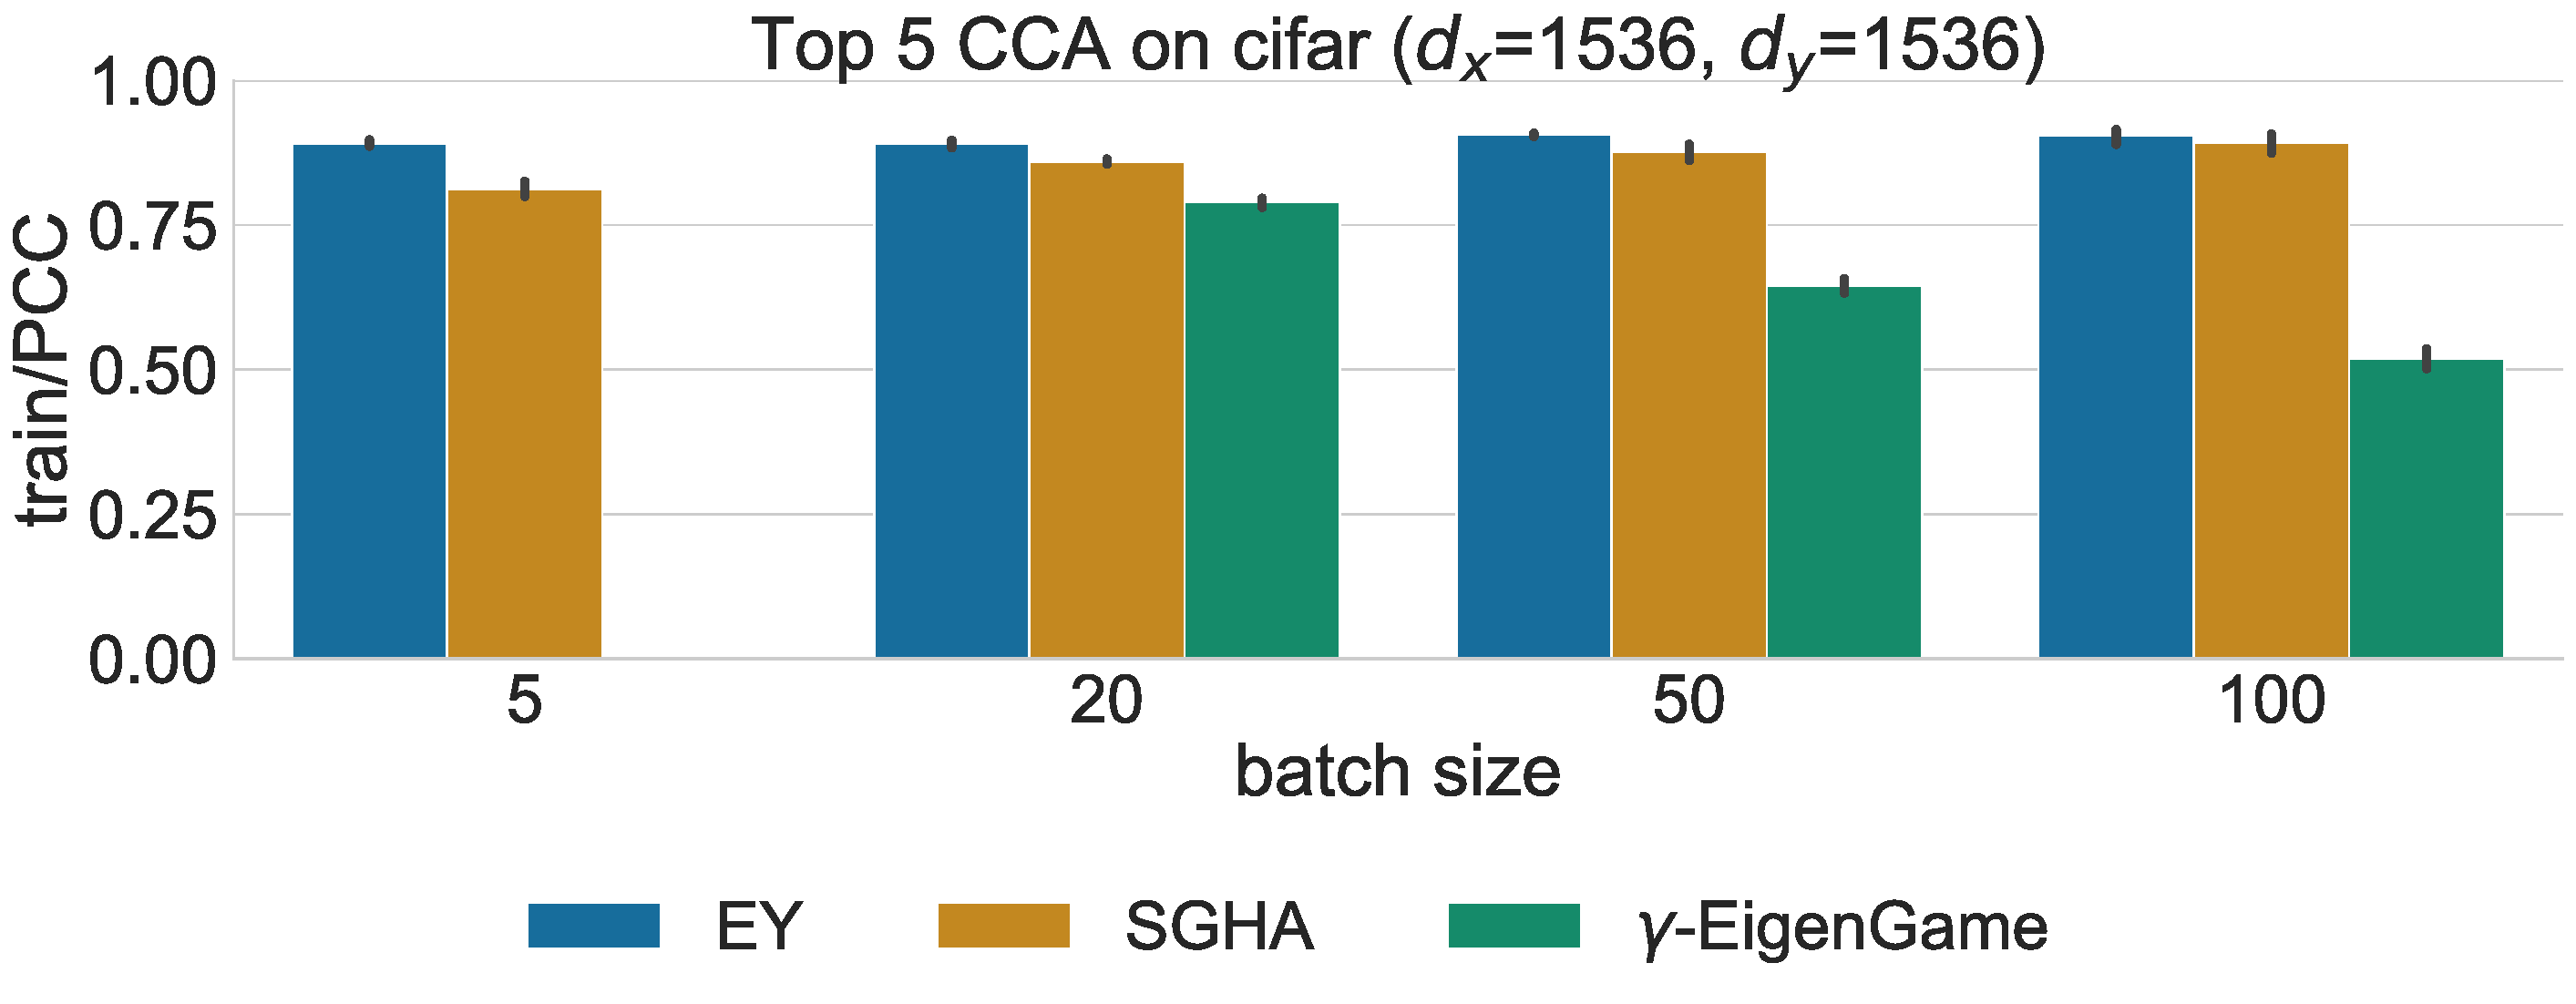
\includegraphics[width=0.8\textwidth]{figures/CCA/cifar_models_different_batch_sizes}
    \caption{Stochastic CCA on CIFAR using PCC: Performance across varying mini-batch sizes. Shaded regions signify \(\pm\) one standard deviation around the mean of 5 runs.}
    \label{fig:corr_cifar}
\end{figure}

\begin{figure}
    \centering
    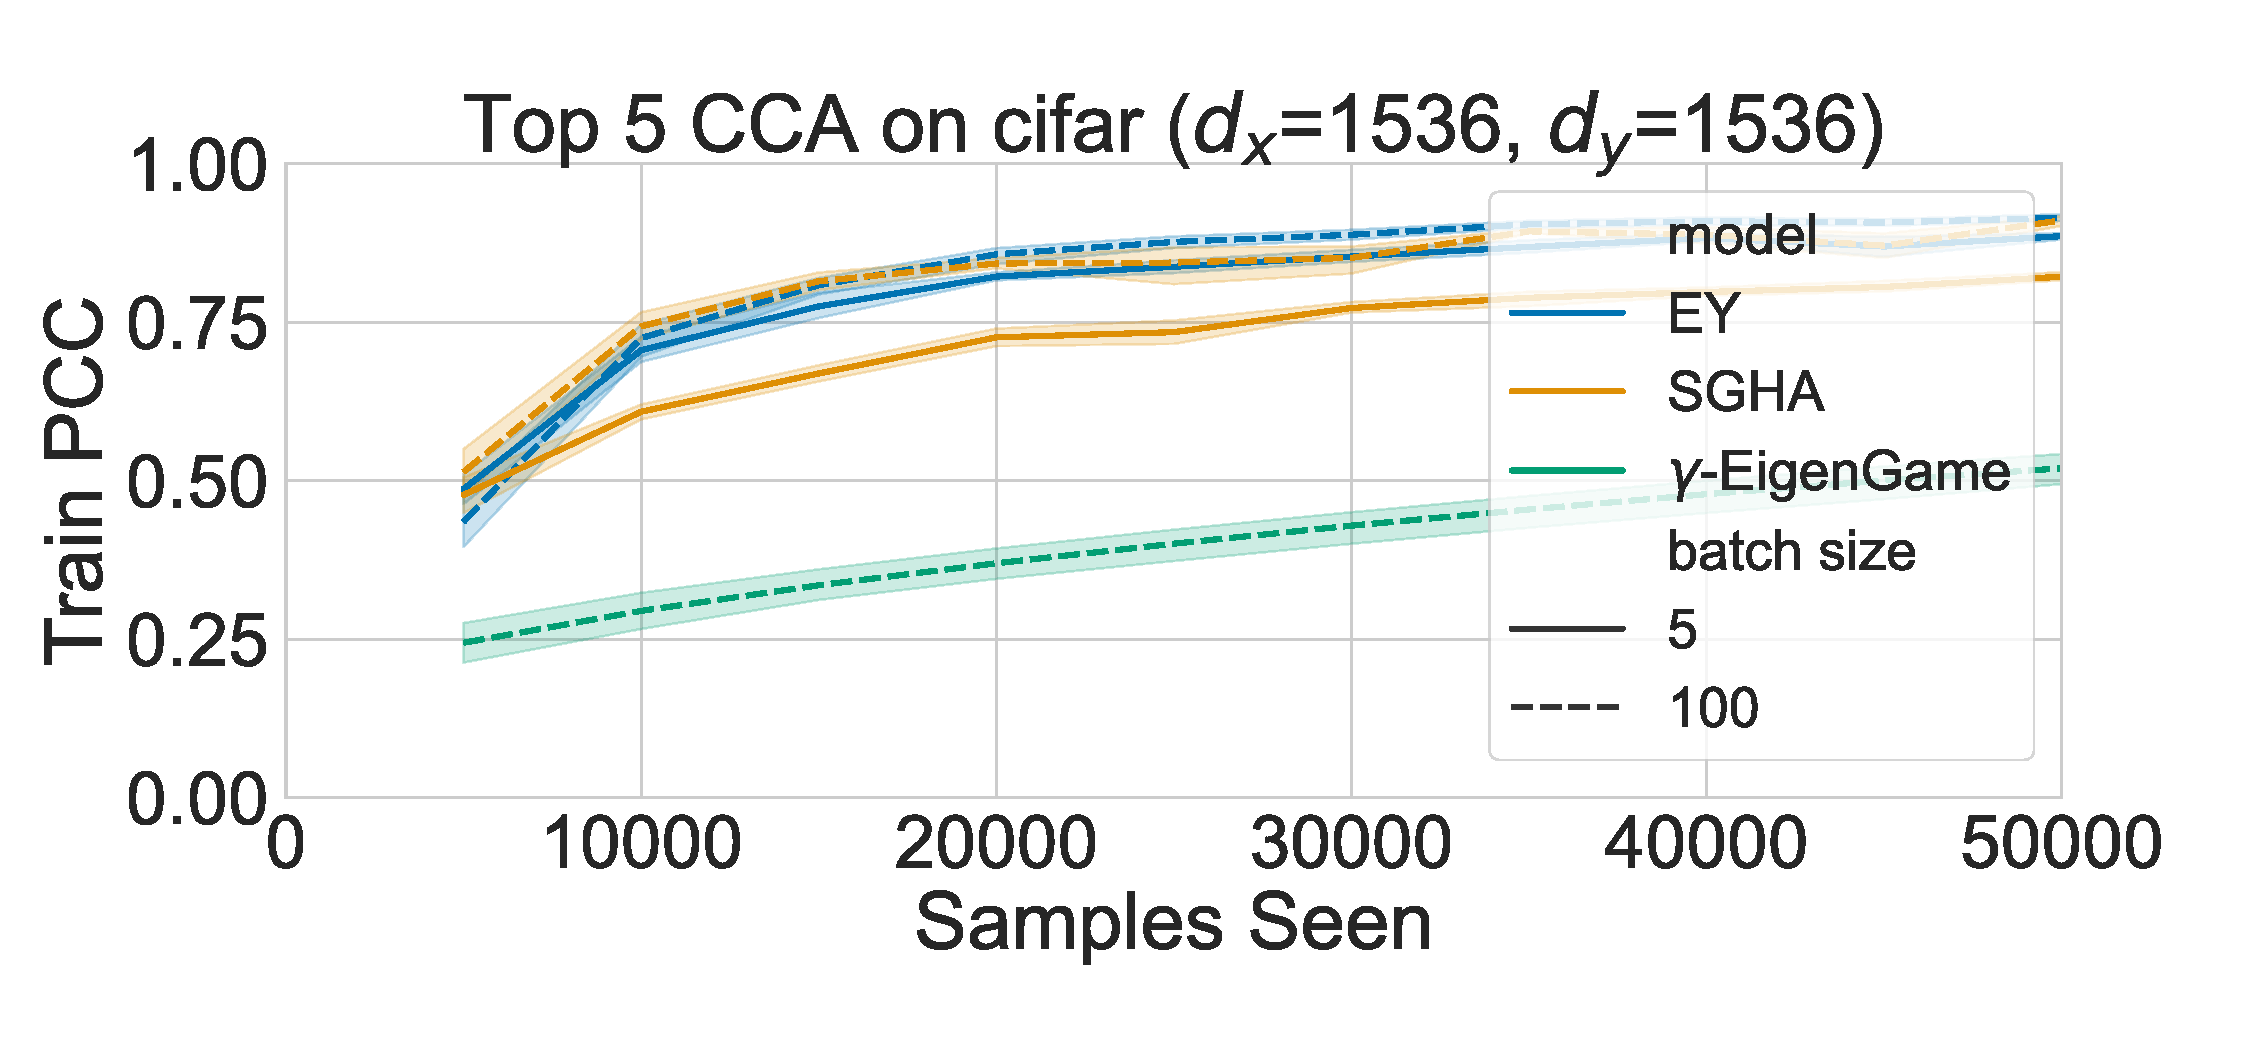
\includegraphics[width=0.8\textwidth]{figures/CCA/cifar_allbatchsizes_pcc}
    \caption{Stochastic CCA on CIFAR: Training progress over a single epoch for mini-batch sizes 5, 100.}
    \label{fig:learningcurve_cifar}
\end{figure}

\subsection{Stochastic PLS UK Biobank}
In this section, we aim to demonstrate the exceptional scalability and efficiency of our Stochastic PLS method, PLS-EY, in handling extremely high-dimensional imaging genetics data.
We employ imaging genetics data from the UK Biobank \citep{sudlow2015uk} as our test bed, given its comprehensive and complex nature.
The UK Biobank dataset presents a unique challenge due to the sheer scale of its genetic data, requiring sophisticated regularization strategies.

PLS is particularly suited for imaging-genetics studies due to its capability to handle high dimensionality and reveal novel phenotypes as well as genetic mechanisms underlying diseases and brain morphometry.
Historically, imaging genetics analyses have been constrained to smaller datasets due to computational limitations \citep{lorenzi2018,Taquet2021,Lefloch2012}.
Moreover, the few studies that have attempted to analyze data of comparable scale to the UK Biobank have typically resorted to partitioning the data into smaller clusters, thereby limiting the scope of their analysis \citep{lorenzi2017secure, altmann2023tackling}.

Our experiment with PLS-EY, conducted on a subset of the UK Biobank dataset consisting of brain imaging data (82 regional volumes) and genetic data (582,565 variants) for 33,333 subjects, is designed to overcome these limitations.
A particular computational challenge we address is maintaining orthogonality between the weight vectors \( u_k \) in the PLS model, which is crucial for the method's effectiveness.
We run PLS-EY with a mini-batch size of 500 and train the GEP-EY PLS analysis for 100 epochs using a learning rate of 0.0001.
This approach allows us to not only manage the high-dimensional nature of the data but also to preserve the integrity and interpretability of the analysis.
To our knowledge, this represents the largest-scale PLS analysis of biomedical data to-date, showcasing the potential of our method to facilitate discoveries in extremely large datasets.

\subsubsection{Data} The UK BioBank data consisted of real-valued continuous brain volumes and ordinal, integer genetic variants.
We used pre-processed (using FreeSurfer \citep{Fischl2012}) grey-matter volumes for 66 cortical (Desikan-Killiany atlas) and 16 subcortical brain regions and 582,565 autosomal genetic variants.
The affects of age, age squared, intracranial volume, sex, and the first 20 genetic principal components for population structure were removed from the brain features using linear regression to account for any confounding effects.
Each brain ROI was normalized by removing the mean and dividing the standard deviation.
We processed the genetics data using PLINK \citep{Purcell2007} keeping genetic variants with a minor allele frequency of at least 1\%  and a maximum missingness rate of 2\%.
We used mean imputation to fill in missing values and centered each variant.
To generate measures of genetic disease risk, we calculated polygenic risk scores using PRSice \citep{PRSice2014}.
We calculated scores, with a p-value threshold of 0.05, using GWAS summary statistics for the following diseases; Alzheimer's \citep{Lambert2013}, Schizophrenia \citep{Trubetskoy2022}, Bipolar \citep{Mullins2021}, ADHD \citep{Demontis2023}, ALS \citep{Van_Rheenen2021}, Parkinson's \citep{Nalls2019}, and Epilepsy \citep{International_League_Against_Epilepsy_Consortium_on_Complex_Epilepsies2018}, using the referenced GWAS studies.

\subsubsection{Observations}
We observed strong validation correlations between all 10 corresponding pairs of representations \( Z^{(1)}_k \) and \( Z^{(2)}_k \) in the PLS model, with weak cross-correlations between \( Z^{(1)}_k \) and \( Z^{(2)}_i \) for \( i \neq k \).
This indicates that our model learned a coherent and orthogonal subspace, as shown in Figure \ref{fig:UKBB_corr}.
Furthermore, the PLS representations \( Z \) were significantly associated with genetic risk measures for several disorders, suggesting that the learned PLS subspace encodes relevant information for genetic disease risk, a critical insight for biomedical research (Figure \ref{fig:genetic_risk}). These results demonstrate the scalability of our method to extremely high-dimensional data, and its ability to learn interpretable representations.

\begin{figure}
    \centering
    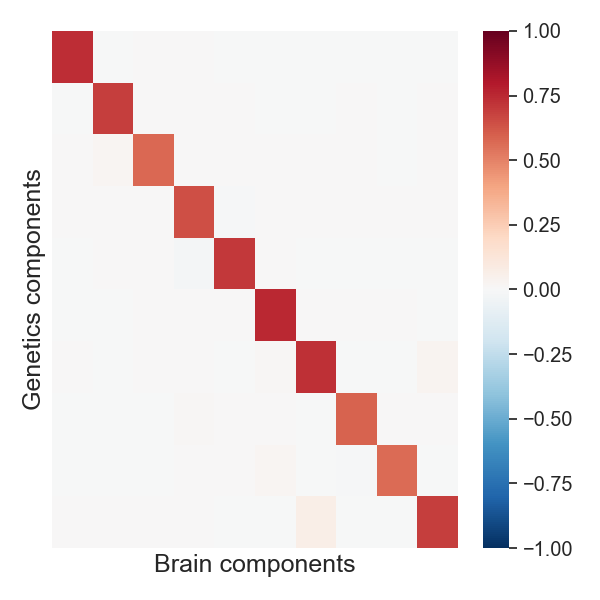
\includegraphics[width=0.6\textwidth,trim={0.8cm 0cm 0.3cm 0cm}]{figures/UKBB/cross_corr.png}
    \caption{Pearson correlations among PLS latent variables \( Z_k \) derived from UK Biobank data.}
    \label{fig:UKBB_corr}
\end{figure}

\begin{figure}
    \centering
    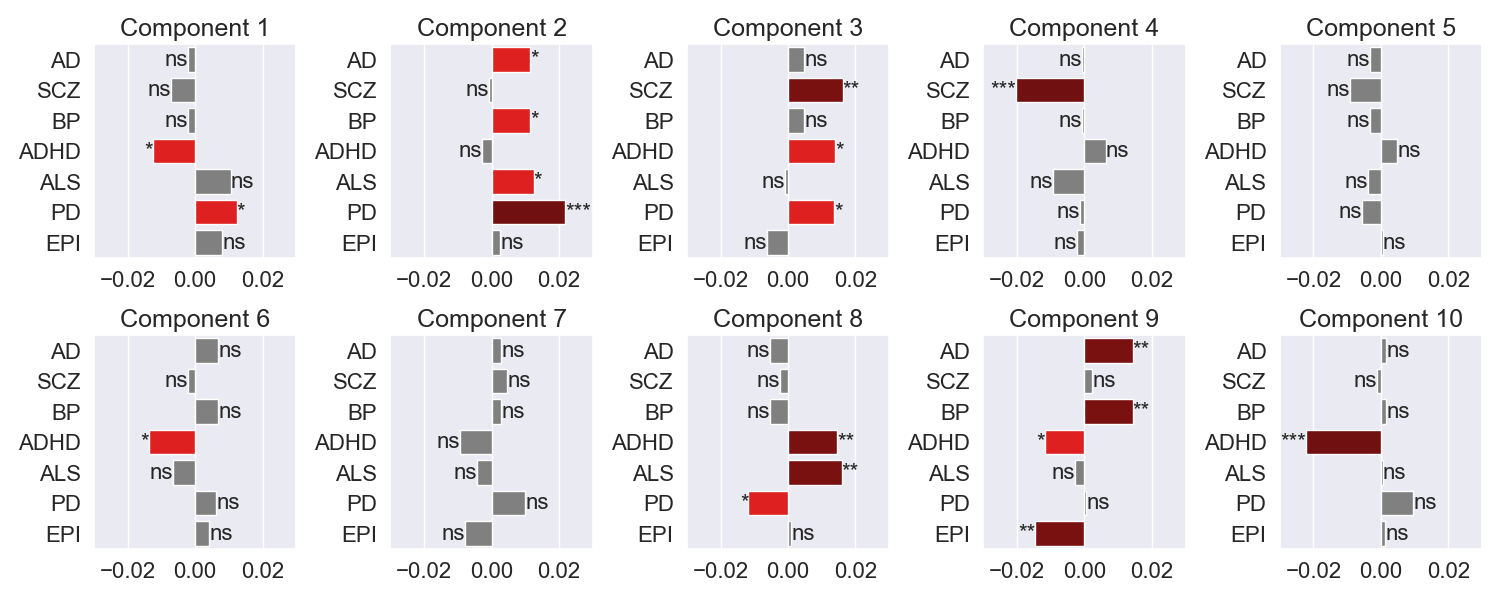
\includegraphics[width=0.99\textwidth,trim={0.5cm 0cm 0.7cm 0cm}]{figures/UKBB/prs_correlations.png}
    \caption{Correlation between PLS brain representations \( Z \) and genetic risk scores for various disorders. AD=Alzheimer's disease, SCZ=Schizophrenia, BP=Bipolar, ADHD=Attention deficit hyperactivity disorder, ALS=Amyotrophic lateral sclerosis, PD=Parkinson's disease, EPI=Epilepsy. $\text{ns}: 0.05< p \leq 1, \ast: 0.01< p \leq 0.05, \ast\ast: 0.001< p \leq 0.01, \ast\ast\ast: 0.0001< p \leq 0.001$.}
    \label{fig:genetic_risk}
\end{figure}

\section{Discussion}

\subsection{Limitations}

This chapter presents a comprehensive exploration and development of novel algorithms for Canonical Correlation Analysis (CCA) and Partial Least Squares (PLS), focusing on scalability and efficiency in high-dimensional and large-scale datasets.
Our approach introduces the Eckhart-Young (EY) inspired objectives for Generalized Eigenvalue Problems (GEPs) and their application in stochastic or data-streaming settings, paving the way for more efficient and scalable solutions to classical subspace learning problems.

Our proposed CCA-EY and PLS-EY methods demonstrate significant advancements over traditional approaches in handling the computational complexity and scalability issues inherent in high-dimensional data.
By reformulating the CCA and PLS objectives, we provide a path to efficiently analyze large datasets, which was previously infeasible due to computational limitations.
The empirical evaluation on diverse datasets, including MediaMill, Split-CIFAR-10, and the UK Biobank, not only validates the effectiveness of our methods but also highlights their superiority in convergence speed and robustness to hyperparameter tuning.

The results from the MediaMill and Split-CIFAR-10 datasets underscore the potential of CCA-EY in achieving faster convergence with minimal hyperparameter tuning, a crucial factor for practical applications.
This advantage is particularly pronounced when comparing our method to established baselines like $\gamma$-EigenGame and SGHA. Additionally, the application of our methods to the UK Biobank dataset represents a breakthrough in the analysis of imaging genetics data, showcasing the capability of PLS-EY to manage extraordinarily high-dimensional data while extracting meaningful and interpretable representations.

Furthermore, our methods' ability to capture relevant information for genetic disease risk, as evidenced in the UK Biobank study, opens new avenues for biomedical research.
The significant associations between the PLS representations and genetic risk measures for various disorders provide valuable insights into the genetic mechanisms underlying diseases and brain morphometry.

\subsection{Future Work}

\subsection{Proximal Gradient Descent for Regularized GEPs}

Our future initiatives will enhance CCA, PCA and PLS by incorporating proximal gradient descent for efficient handling of complex regularization terms. This methodology is ideally suited for scenarios where the loss function comprises a smooth, differentiable component plus a non-smooth regularization term. The proximal gradient technique utilizes a gradient step followed by a proximal step, enabling effective management of non-smooth penalties such as L1-norm or Total Variation (TV), which are instrumental in enforcing sparsity and structural constraints.

\subsubsection{Objective Formulation with Regularization}

We aim to modify the CCA framework by integrating specific regularization terms directly into the loss function of the Generalized Eigenvalue Problem (GEP). The revised loss function, denoted as $\mathcal{L}_{\text{Proximal CCA-EY}}(\mathbf{U}_1, \mathbf{U}_2)$, will incorporate the regularization terms $R_1(\mathbf{U}_1)$ and $R_2(\mathbf{U}_2)$, enabling the optimization of CCA with additional constraints. The objective function for Proximal CCA-EY will be defined as:

\begin{align*}
    \mathcal{L}_{\text{Proximal CCA-EY}}(\mathbf{U}_1, \mathbf{U}_2) &= \mathcal{L}_{\text{EY}}(\mathbf{U}_1, \mathbf{U}_2)
    + \lambda_1 R_1(\mathbf{U}_1) + \lambda_2 R_2(\mathbf{U}_2),
\end{align*}

where $\mathcal{L}^{\text{Proximal CCA-EY}}$ represents the Proximal CCA-EY loss function, $\lambda_1$ and $\lambda_2$ are regularization parameters, and $R_1(\mathbf{U}_1)$ and $R_2(\mathbf{U}_2)$ are the regularization terms for each view.

\subsubsection{Proximal Gradient Descent Mechanism}

The proximal gradient updates for this augmented CCA formulation are specified as:

\begin{align}
\mathbf{U}1^{(t+1)} &= \text{prox}{\alpha \lambda_1 R_1}(\mathbf{U}_1^{(t)} - \alpha \nabla{\mathbf{U}_1} \mathcal{L}^{\text{EY}}(\mathbf{U}_1^{(t)}, \mathbf{U}_2^{(t)})), \
\mathbf{U}2^{(t+1)} &= \text{prox}{\alpha \lambda_2 R_2}(\mathbf{U}_2^{(t)} - \alpha \nabla{\mathbf{U}_2} \mathcal{L}^{\text{EY}}(\mathbf{U}_1^{(t)}, \mathbf{U}_2^{(t)})),
\end{align}

where $\text{prox}_{\alpha \lambda_i R_i}(\mathbf{v})$ denotes the proximal operator for the regularization term $R_i$ with parameter $\lambda_i$, and $\alpha$ represents the learning rate. Note that the gradients $\nabla{\mathbf{U}_1} \mathcal{L}^{\text{EY}}(\mathbf{U}_1^{(t)}, \mathbf{U}_2^{(t)})$ and $\nabla{\mathbf{U}_2} \mathcal{L}^{\text{EY}}(\mathbf{U}_1^{(t)}, \mathbf{U}_2^{(t)})$ are computed only for the smooth part of the loss function, i.e., $\mathcal{L}^{\text{EY}}(\mathbf{U}_1, \mathbf{U}_2)$, and do not include the regularization terms.

The proximal operator is defined as solving:

\begin{align*}
\text{prox}{\alpha \lambda_i R_i}(\mathbf{v}) = \arg \min\mathbf{u} \left( R_i(\mathbf{u}) + \frac{1}{2\alpha} |\mathbf{u} - \mathbf{v}|_2^2 \right).
\end{align*}

This update effectively balances the influence of the gradient of the smooth loss function and the geometry imposed by the regularization, making the approach robust to the inclusion of complex constraints in the optimization of CCA.

\subsubsection{Efficiency and Applicability}

The proximal gradient descent method excels in large-scale optimization challenges where traditional techniques struggle due to the presence of non-smooth terms. By separating the optimization of the smooth component from the non-smooth regularization, proximal steps can be efficiently computed, particularly when $R_i$ allows a straightforward proximal formulation.

\subsection{Conclusion}

In summary, this chapter contributes to the fields of machine learning and multiview data analysis by introducing scalable and efficient solutions for CCA and PLS, applicable in a variety of domains, including but not limited to neuroimaging and genetics.
Our work not only addresses significant computational challenges but also lays the groundwork for future research and practical applications in analyzing large-scale, high-dimensional datasets.